\documentclass[10pt]{article}
\usepackage[a4paper, margin=2cm]{geometry}
\usepackage{amsmath}
\usepackage{amsfonts} 
\usepackage{booktabs}
\usepackage{bm}
\usepackage{enumitem}
\usepackage{graphicx}
\usepackage[justification=centering]{caption}
\usepackage{xcolor}
\usepackage{hyperref}
\hypersetup{colorlinks=true, allcolors=blue}
\urlstyle{sf}
\usepackage{mdframed}
\usepackage{listings}
\mdfdefinestyle{default}{linecolor=black, linewidth=1.2pt}
\title{NEGFtrans User Manual}
\author{Yi-Cheng Lin}
\date{\today}
\setlist{listparindent=\parindent}
\lstset{frame=lines, showlines=true}
\newcommand{\toc}[1]{\phantomsection\addcontentsline{toc}{subsubsection}{#1} #1}

\begin{document}
\maketitle

\tableofcontents

\section{Introduction}
As shown in Figure 1, the physical system we're dealing with is the scattering region between two reservoir, where the reservoir is assumed to have flat potential with the value being $V_L$ (V{\_}L) and $V_R$ (V{\_}R) respectively, so that at the boundary can be matched by assuming there's only plane wave in the reservoir. As for the scattering region: $0 \le z \le L_z$(L{\_}Z), the potential is given by $V(\bm{r})$(data in POTENTIAL file). In most case, one should make sure that $V(x, y, 0) = V_L$ and $V(x, y, L_z) = V_R$ so that the potential profile of the system do not have abrupt change at the boundary. Also, $\mu$ (MU) represent the Fermi-energy level relative to the potential profile.

\begin{figure}[h!]
\centering
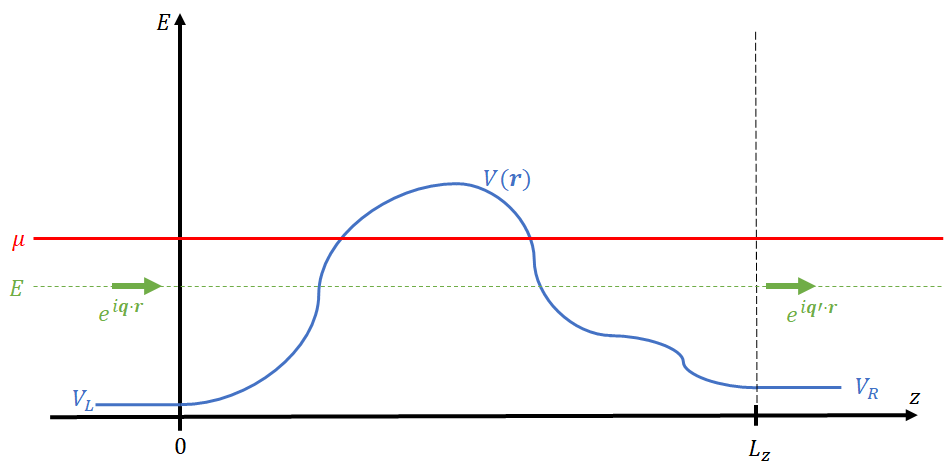
\includegraphics[width=0.8\textwidth]{profile}
\caption{Schematic profile of the physical system}
\end{figure}

\noindent
In xy-direction, the physical system is assumed to be periodic. If you want to make it non-periodic, just mimic the situation by enlarge the cell at that dimension as you did in VASP, and put some smooth barrier at the boundary. Since the program expand the wavefunction into plane wave in xy-direction, you should avoid sharp changes of $V(\bm{r})$ in xy-direction.\\\\
Once you obtain the transmission coefficient $\tau(E)$, the current can be calculated by Landauer formula
\[I = \frac{2e}{h}\int dE\ \tau(E) (f_L - f_R)\]
Note that the transmission coefficient is a dimensionless function. Also note that the current has dimension [charge / time], so it is defined as the current through the $L_x \times L_y$ cross-section area. If you want to calculate the current density, you should use the following formula
\begin{align*}
J &= \frac{I}{L_x L_y} && \text{Periodic crystal in both x and y direction} \\
J &= \frac{I}{L_x} && \text{2D crystal, periodic in x direction (surface current density)} 
\end{align*}

\section{Input Files}
Two files need to be prepared in the same directory where you submit the job. The format are explained as follow:
\subsection{INPUT}
The INPUT file is in Fortran namelist format. Thus, the file should look like
\begin{lstlisting}
&INPUT
if_transmission = .true.
LX = 10.0
LY = 8.0
LZ = 20.0
! This is comment
TRANSMISSION_GRID = 4.0 20.0 200
...
...
/

\end{lstlisting}
Note that there must be one extra blank line after "/" so that the file can be read successfully. The "!" sign is for comment. The parameters can be assigned without ordering, and each assignment must be separated by either "comma" or "newline" or "space". And the value of an array input (e.g. TRANSMISSION{\_}GRID) should be separated by "space" (e.g. 4.0 20.0 200). For more about namelist, google for it or take a look at this: \url{https://jules-lsm.github.io/vn5.1/namelists/intro.html}\\\\
The meaning of the parameters are listed as follow, the value indicate the initial value, and those with * sign means that the parameter must be specified. Also, note that at least one of if{\_}xxx must be set to .true. , otherwise there's nothing to calculate.

\begin{itemize}
\item \toc{if{\_}density} = .false.\\
Determine whether to calculate the density of the given POTENTIAL input. If set 
\begin{center}
if{\_}density = .true.
\end{center}
Then the output file DENSITY will be generated.
\item \toc{if{\_}transmission} = .false.\\
Determine whether to calculate the transmission coefficient of the given POTENTIAL input. If set 
\begin{center}
if{\_}transmission = .true.
\end{center}
Then the output file TRANSMISSION will be generated.
\item \toc{if{\_}LDOS} = .false.\\
Determine whether to calculate the Local Density Of State of the given POTENTIAL input. If set 
\begin{center}
if{\_}LDOS = .true.
\end{center}
Then the output file LDOS will be generated.
\item \toc{V{\_}L} = 0.0 (eV)\\
The potential bottom of the free electron gas at left boundary. In most case, it should match the leftmost value of your POTENTIAL input file.
\item \toc{V{\_}R} = 0.0 (eV)\\
The potential bottom of the free electron gas at right boundary. In most case, it should match the rightmost value of your POTENTIAL input file.
\item \toc{MU} = 5.568 (eV)\\
Useful only when (if{\_}density = .true.). The Fermi-energy of the system. If not specified, it's set to the Fermi-energy of free-electron gas with $r_s = 3.0$ bohr (i.e. Wigner–Seitz radius of Au).
\item \toc{ETA} = 1E-5 (Hartree)\\
The retarded Green's function is defined by $G_+ = ((E+i\eta)\hat{I}-\hat{H_0}-\hat{\Sigma}_R-\hat{\Sigma}_L)^{-1}$, with ETA=$\eta$.
\item \toc{TEMPERATURE} = 20.0 (K)\\
Useful only when (if{\_}density = .true.). The temperature of the system. However, this only affect the Fermi-Dirac distribution, so note that this do not include all the temperature effect of the physical system.
\item \toc{LX} = none* (\AA)\\
The size of the box (supercell) in x-direction.
\item \toc{LY} = none* (\AA)\\
The size of the box (supercell) in y-direction.
\item \toc{LZ} = none* (\AA)\\
The size of the box (supercell) in z-direction, which is the transport direction.
\item \toc{ENCUT} = 100.0 (eV)\\
The parameters that determine how large our plane wave basis is. If we express the plane wave by $(e^{\bm{G}\cdot\bm{r}})$, then $\bm{G}$ is restricted by 
\[\frac{\hbar^2 |\bm{G}|^2}{2m_e} \le E_{cut}\]
where ENCUT$=E_{cut}$, and $m_e$ is the mass of electron.
\item \toc{GAP} = 6.0 (unit in $k_B T$)\\
Determine the upper and lower bound of the line-integral near Fermi-energy. There's no need to change this value in most case.
\item \toc{VDS} = 0.0 (eV)\\
Currently useless, there's no support for the calculation of non-equilibrium density in this version.
\item \toc{TRANSMISSION{\_}GRID} = none none none (eV, eV, integer)\\
For (if{\_}transmission = .true.) , this parameter must be specified. This parameter is a 3-element array: 
\begin{center}
TRANSMISSION{\_}GRID = $E_{min}\ E_{max}\ N_E$
\end{center}
where the energy grid for transmission coefficient is given by
\[E_i = E_{min} + \left(\frac{E_{max} - E_{min}}{N_E}\right) (i - 1) \qquad i=1...N_E\]
Note that the last point will NOT be included. For example, for 
\begin{center}
TRANSMISSION{\_}GRID = 0.0 2.0 4
\end{center}
then the energy grid will be
\[\{E_i\} = 0.0, 0.5, 1.0, 1.5\]
\item \toc{LDOS{\_}ENERGY{\_}GRID} = none none none (eV, eV, integer)\\
For (if{\_}LDOS = .true.) , this parameter must be specified. This parameter is a 3-element array, and the layout is the same as TRANSMISSION{\_}GRID.
\item \toc{LDOS{\_}GRID} = none none none (integer, integer, integer)\\
For (if{\_}LDOS = .true.) , this parameter must be specified. This parameter is a 3-element array:
\begin{center}
LDOS{\_}GRID = $m_x\ m_y\ m_z$
\end{center}
and the meaning of the integer is interpreted as (take $m_x$ for example)
\[ m_x =
\begin{cases}
-1 & \text{integrate over x-direction by} \int_{0}^{L_x} dx\ LDOS(x, y, z, E) \\\\
0 & \text{write out all the value of LDOS in x-direction}\\\\
\text{others} &\text{take the } (m_x)^{th} \text{ x-grid point. The real-space grid is the same as POTENTIAL}\\
 & \text{input, with Fortran index convention ([index of first grid point] = 1)}
\end{cases}\]
For example, for
\begin{center}
LDOS{\_}GRID = -1 5 0
\end{center}
We'll have
\[LDOS(z, E) = \int_{0}^{L_x} dx\ LDOS(x, y_5, z, E)\]
Another example, if we set
\begin{center}
LDOS{\_}GRID = -1 -1 -1
\end{center}
Then it become position-independent, which is exactly Density Of State (DOS)!
\item \toc{NGX} = auto-determined (integer)\\
Determine the number of grid point in reciprocal space in x-direction. There's no need to change this value in most case.
\item \toc{NGY} = auto-determined (integer)\\
Similar to NGX, but in y-direction.
\item \toc{NKX} = none* (interger)\\
Determine the number of Bloch k-point in x-direction, and the Monkhorst-Pack mesh is used in my program. If the physical system is not assumed periodic in x-direction, then simply set NKX = 1.
\item \toc{NKY} = none* (interger)\\
Similar to NKX, but in y-direction.
\item \toc{N{\_}circle} = 40 (points/$\pi$)\\
The number of integration points of the hemi-circle integral. There's no need to change this value in most case.
\item \toc{N{\_}line{\_}per{\_}eV} = 500 (points/eV)\\
The density of integration points of the line integral near Fermi-energy. There's no need to change this value in most case.
\end{itemize}

\subsection{POTENTIAL}
The POTENTIAL should be prepared in the following format:
{\footnotesize
\begin{lstlisting}
   50   90  300
    21.000000        21.000000        21.000000        21.000000        21.000000    
    21.000000        21.000000        21.000000        21.000000        21.000000    
    21.000000        21.000000        21.000000        21.000000        21.000000    
    19.593163        15.481018        11.852654        8.7080724        6.0472725    
    3.8702544        2.1770181       0.96756365       0.24189095       0.50044916E-07
   0.24189095       0.96756365        2.1770181        3.8702544        6.0472725    
    8.7080724        11.852654        15.481018        19.593163        21.000000 
                                           ...
\end{lstlisting}
}
\noindent
where the first line should contain three integer represent
\[N_x\ N_y\ N_z\]
(Number of grid-point in x, y, z direction)\\\\
And the 3D array of potential should be flatten out into 1D array by Fortran convention (x in inner loop, z in outer loop), then written into POTENTIAL with 5 values per-line (start from second line). Note that the unit of potential value should be (eV).\\\\
As an example, if you're using Fortran to construct the potential, then you can write out the POTENTIAL file by the following code (assume that potential is stored in the array \texttt{POT}):
\begin{lstlisting}
open(unit=17, file="POTENTIAL")
write(17, '(3I5)') N_x, N_y, N_z
write(17, '(5G17.8)') (((POT(i, j, k), i=1, N_x), j=1, N_y), k=1, N_z)
\end{lstlisting}

\section{Output Files}
\subsection{OUTPUT}
The OUTPUT file contains all the information during the calculation, including parameters (so that you may check whether INPUT file is read properly), size of the plane wave basis, k-point grid, total charge (for if{\_}density = .true.), and CPU time. You can also check whether the program executed successfully by looking at the end of OUTPUT file. If success, it will print
\begin{lstlisting}
 ********************
 *                  *
 *      DONE        *
 *                  *
 ********************
\end{lstlisting}
\vspace{1em}
Note that the format of INPUT parameter will be slightly different for array input. For example, in INPUT file
\begin{lstlisting}
...
LDOS_GRID = -1 0 0
...
\end{lstlisting}
Then the OUTPUT file will print (2*0 represent two zero in a row)
\begin{lstlisting}
 ...
 LDOS_GRID=-1         , 2*0          ,
 ...
\end{lstlisting}

\subsection{DENSITY}
For (if{\_}density = .true.), the DENSITY file will be generated. Similar to the format of POTENTIAL input file, the first line contain three integer that represent
\[N_x\ N_y\ N_z\]
(Number of grid-point in x, y, z direction, same as POTENTIAL file)\\\\
The number density calculated by this program is a 3D array, the unit is ($\text{\AA}^{-3}$), and it will be first flatten out into 1D array by Fortran convention (x in inner loop, z in outer loop), then written into DENSITY file with 5 values per-line (start from second line). More precisely, it is written out by the following Fortran code
\begin{lstlisting}
open(unit=18, file="DENSITY")
write(18, '(3I5)') N_x, N_y, N_z
write(18, '(5G17.8)') (((Density(i, j, k), i=1, N_x), j=1, N_y), k=1, N_z)
\end{lstlisting}

\subsection{TRANSMISSION}
For (if{\_}transmission = .true.), the TRANSMISSION file will be generated. This file is in (.dat) format. The energy is in unit (eV), and the transmission coefficient is dimensionless. With this file you can obtain $\tau (E)$, that is, the transmission coefficient as a function of energy.

\subsection{LDOS}
For (if{\_}LDOS = .true.), the LDOS file will be generated. The unit is ($\text{\AA}^{-n} \text{eV}^{-1}$), where 
\[n \equiv 3 - [\text{number of -1 in the input parameter LDOS{\_}GRID}]\]
This is because for each dimension being integrated out, the unit will change by a factor of \AA .\\\\
Similar to the format of POTENTIAL input file, the first line contain four integer that represent
\[M_x\ M_y\ M_z\ M_E\]
(Number of grid-point in x, y, z direction, and the last one is the number of energy grid point. They may be different from POTENTIAL file if any of the dimension is integrated out)\\\\
The number density calculated by this program is a 4D array [x, y, z, E] (E represent energy), and it will be first flatten out into 1D array by Fortran convention (x in inner loop, E in outer loop), then written into LDOS file with 5 values per-line (start from second line). More precisely, it is written out by the following Fortran code
\begin{lstlisting}
open(unit=20, file="LDOS")
write(20, '(4I5)') M_x, M_y, M_z, M_E
write(20, '(5G17.8)') ((((LDOS(i, j, k, i_E), i=1, M_x), j=1, M_y),&
k=1, M_z), i_E=1, M_E)
\end{lstlisting}




\end{document}
